As stated in chapter \ref{chp:dev_goals}  one goal for the project is the creation of system structure with a formal and clean development process. One aspect of this approach is the creation of an abstract system structure before any considerations towards the platform or the implementation details have been made. The sole basis for the system structure shown in this chapter are the requirements listed in the chapters \ref{chp:requirements} and \ref{chp:dev_goals}.\\
Figure \ref{high_level_design} describes  the high level structure of the system. The design should be self explanatory. It implements the classical software paradigm of a distinction between three main system parts: user interface, application logic and data-storage. Note that all platform specific calls and interaction are abstracted through the data-storage module. The application-logic module doesn't need any information about the platform itself. 
\begin{figure}[h!]
\centering
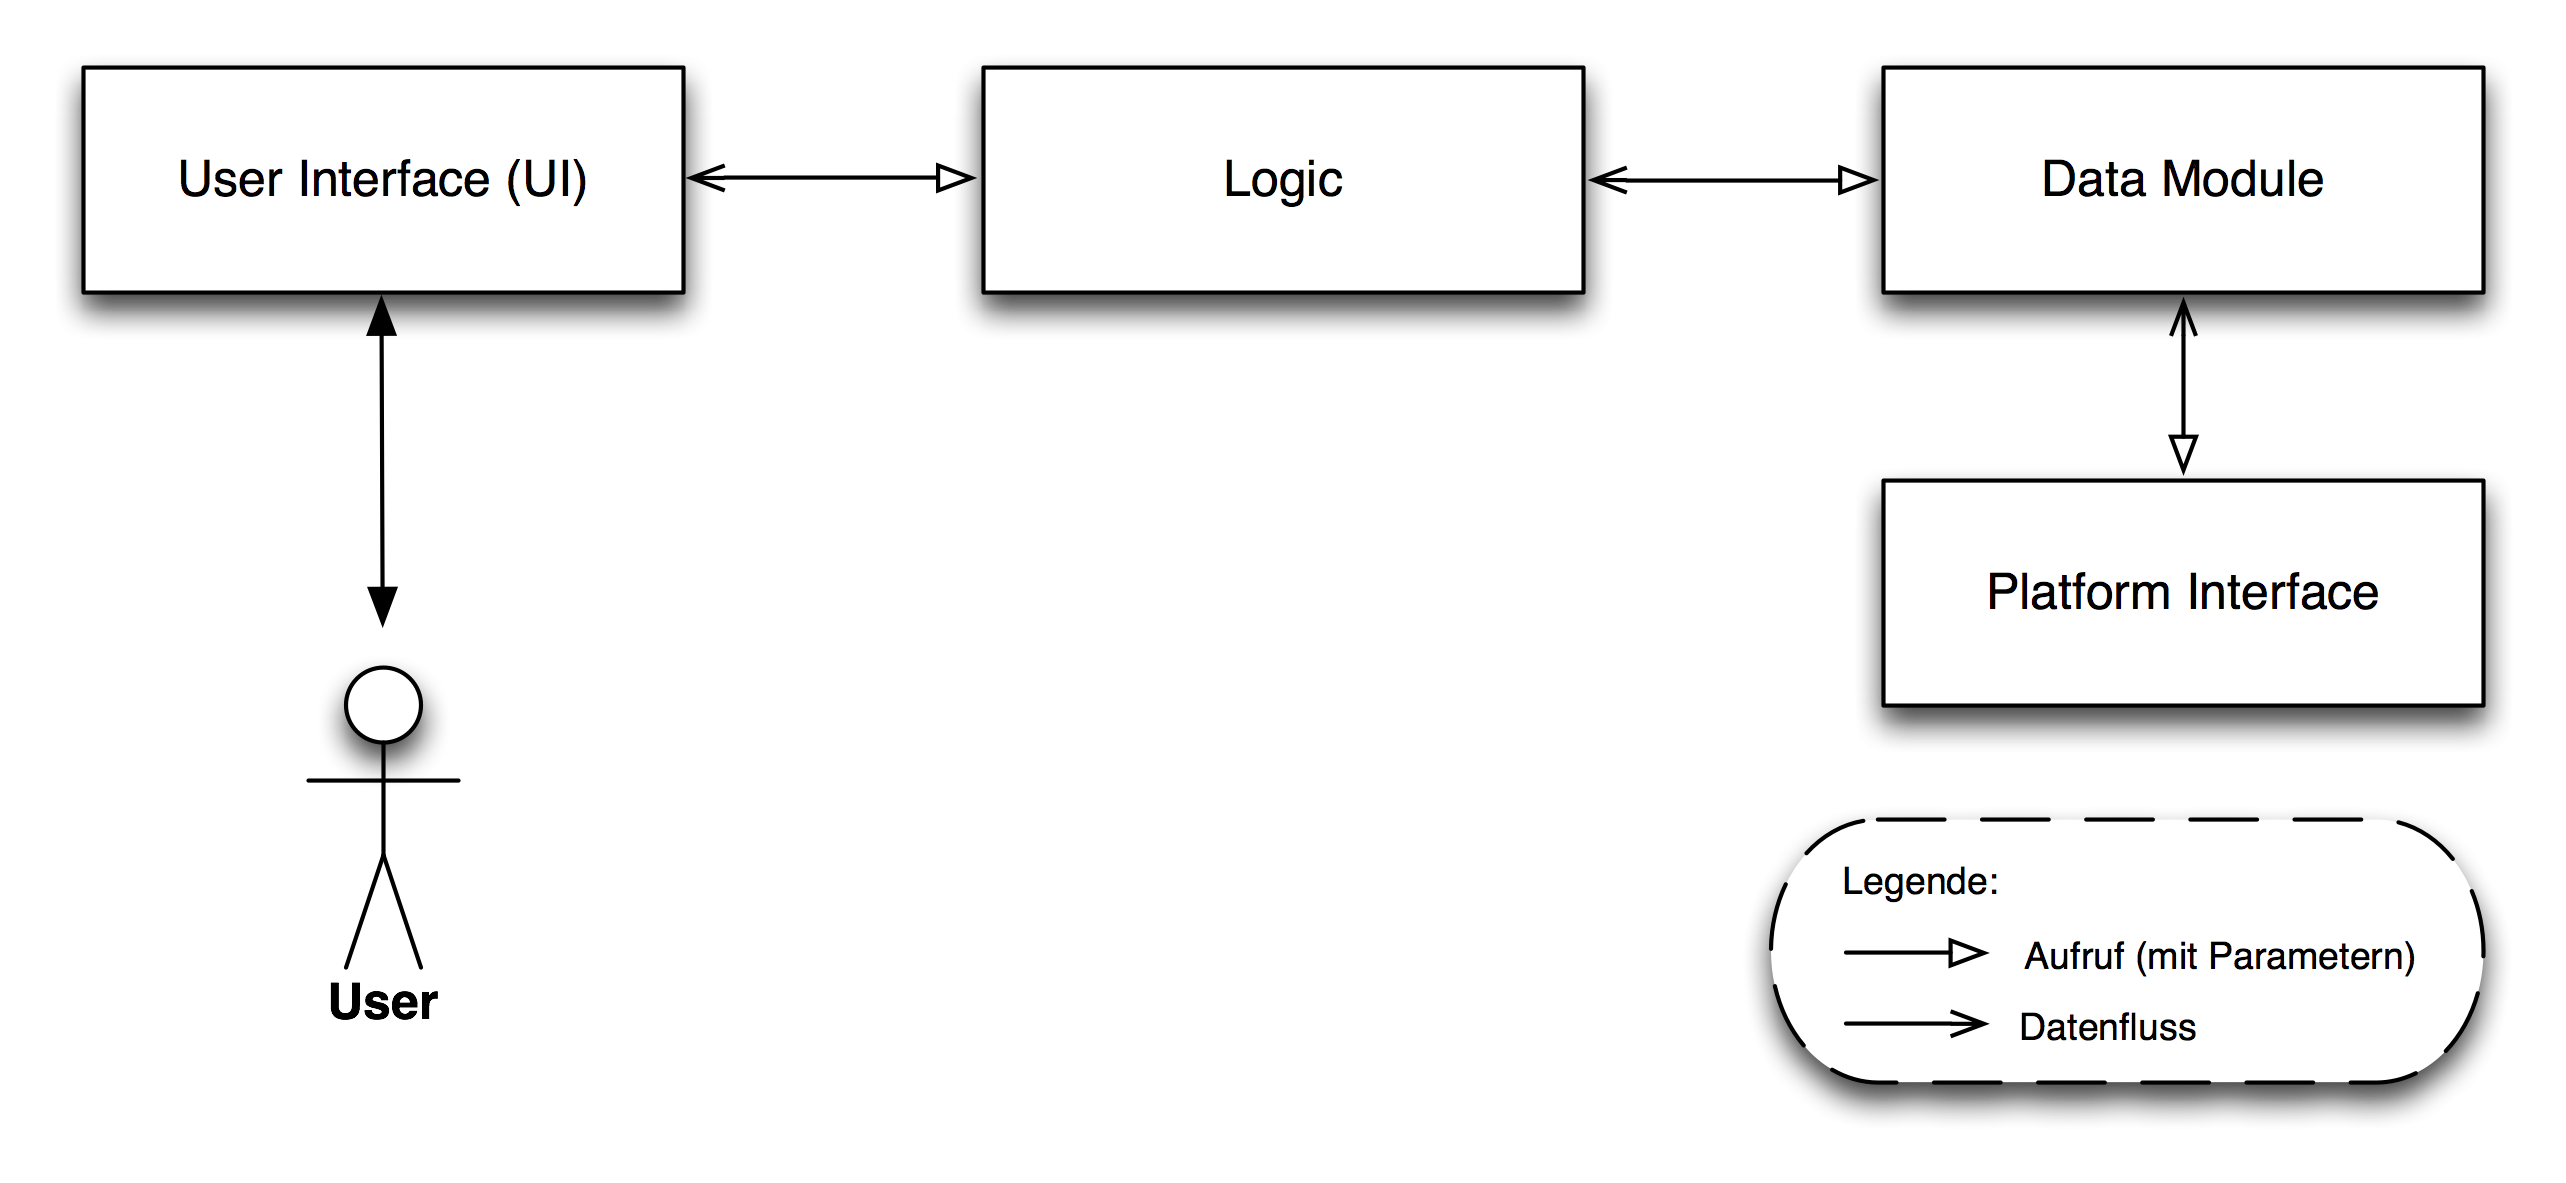
\includegraphics[width=16cm]{pics/top_level_design.png}
\caption{High level design of the system components}
\label{high_level_design}
\end{figure}
In figure \ref{logic} the inner structure of the application-logic is described. The sub-systems shown here are:
\begin{itemize}
\item Event Stuff: This module contains the main functionality of the software. It is described in details in figure \ref{event_stuff}.
\item Event Stuff Tools: This is a collection of helper-functions that solve common tasks for the Event Stuff module.
\item Routing: The routing engine and map-data management are located in this module, separated from the Event Stuff to reduce complexity and to impose the necessity to define clean interface between these system-parts
\item UI Manager: This as an Abstraction of the concrete implementation of the user interface. The Event Stuff module tells the UI-Manager about events that occur and the  UI Manager decides wether and how the user is to be made aware of the situation. With this abstraction the application can look and behave in completely different ways depending an the runtime-configuration of the UI Manager.  
\end{itemize}
\begin{figure}[h!]
\centering
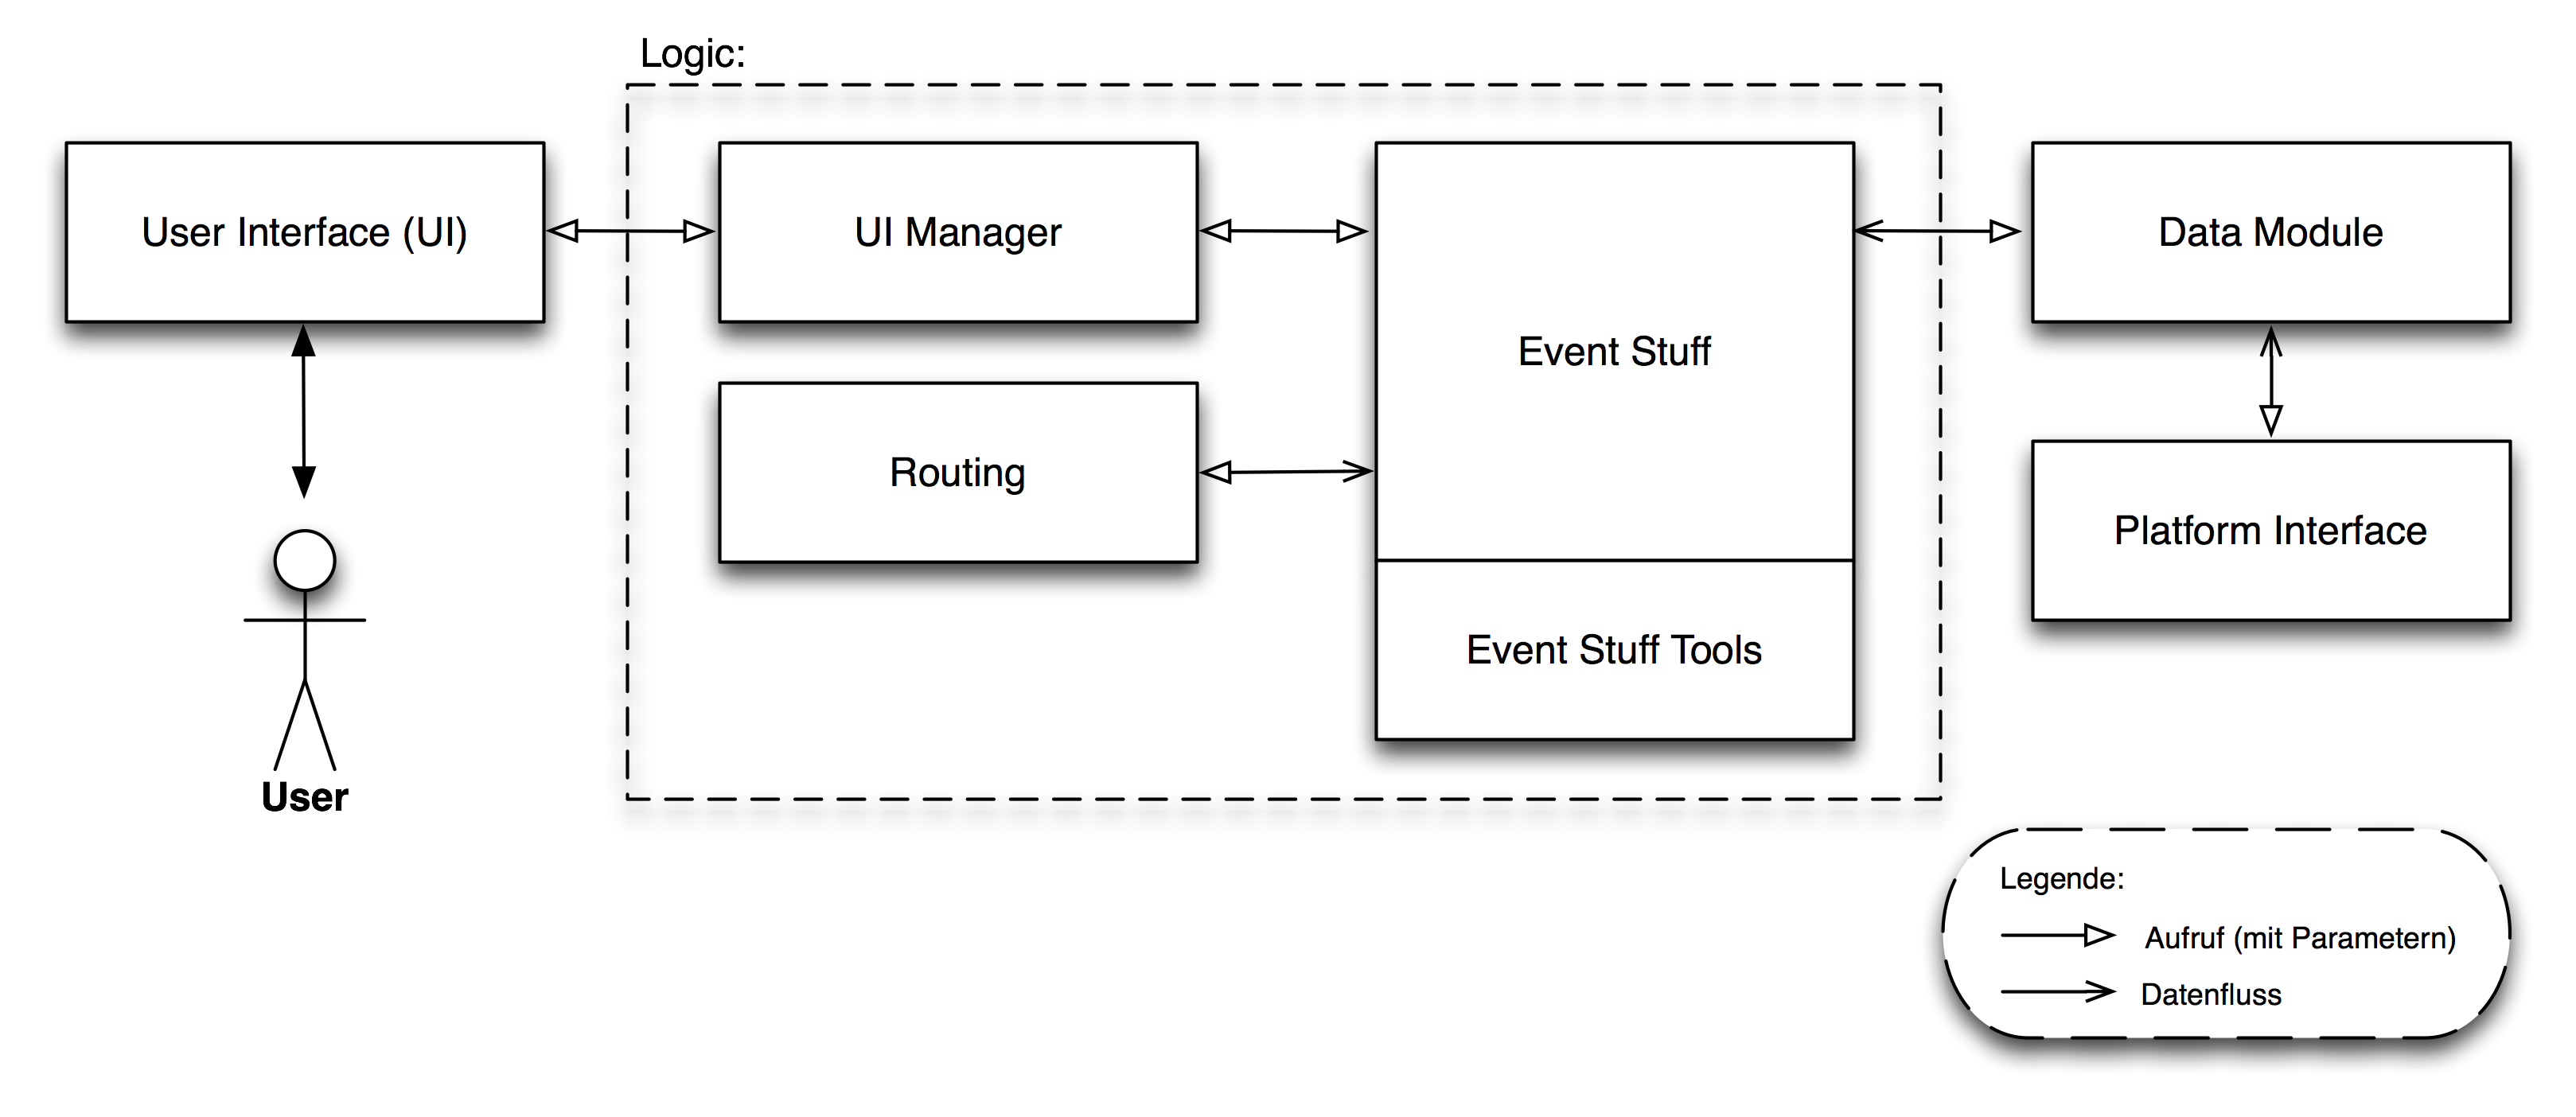
\includegraphics[width=16cm]{pics/logic.png}
\caption{Representation of the logical system elements}
\label{logic}
\end{figure}
Figure  \ref{event_stuff} shows the inner elements of the Event Stuff module. The functionality is divided into these modules:
\begin{itemize}
\item Event Warner: This module needs to run in the background it checks wether the current dayplan can be sustained, given the current position of the user in time and space. It informs the user when he hast to get going in order to meet his next appointment.
\item Plan Bauer: This module is used to create dayplans from the events and the tasks in the database.
\item Plan Optimierer: This module can optimize the current dayplan by inserting executable tasks into the dayplan at practical locations.
\item Termin Vorschkaeger: This module can be used to suggest practical locations and times for meeting between two users of this application. This can only work, when the dayplans of these two users are shared.
\item Erreichbarkeitspruefer: This module is part of the Event Stuff Tools. It can check, wether a given appointment can be reached, given a certain current point in time and space.
\item Time-Finder and Time-Filler: These are helper modules that can suggest a place and a time for a certain task to become an event of a certain deyplan. 
\end{itemize}
\begin{figure}[h!]
\centering
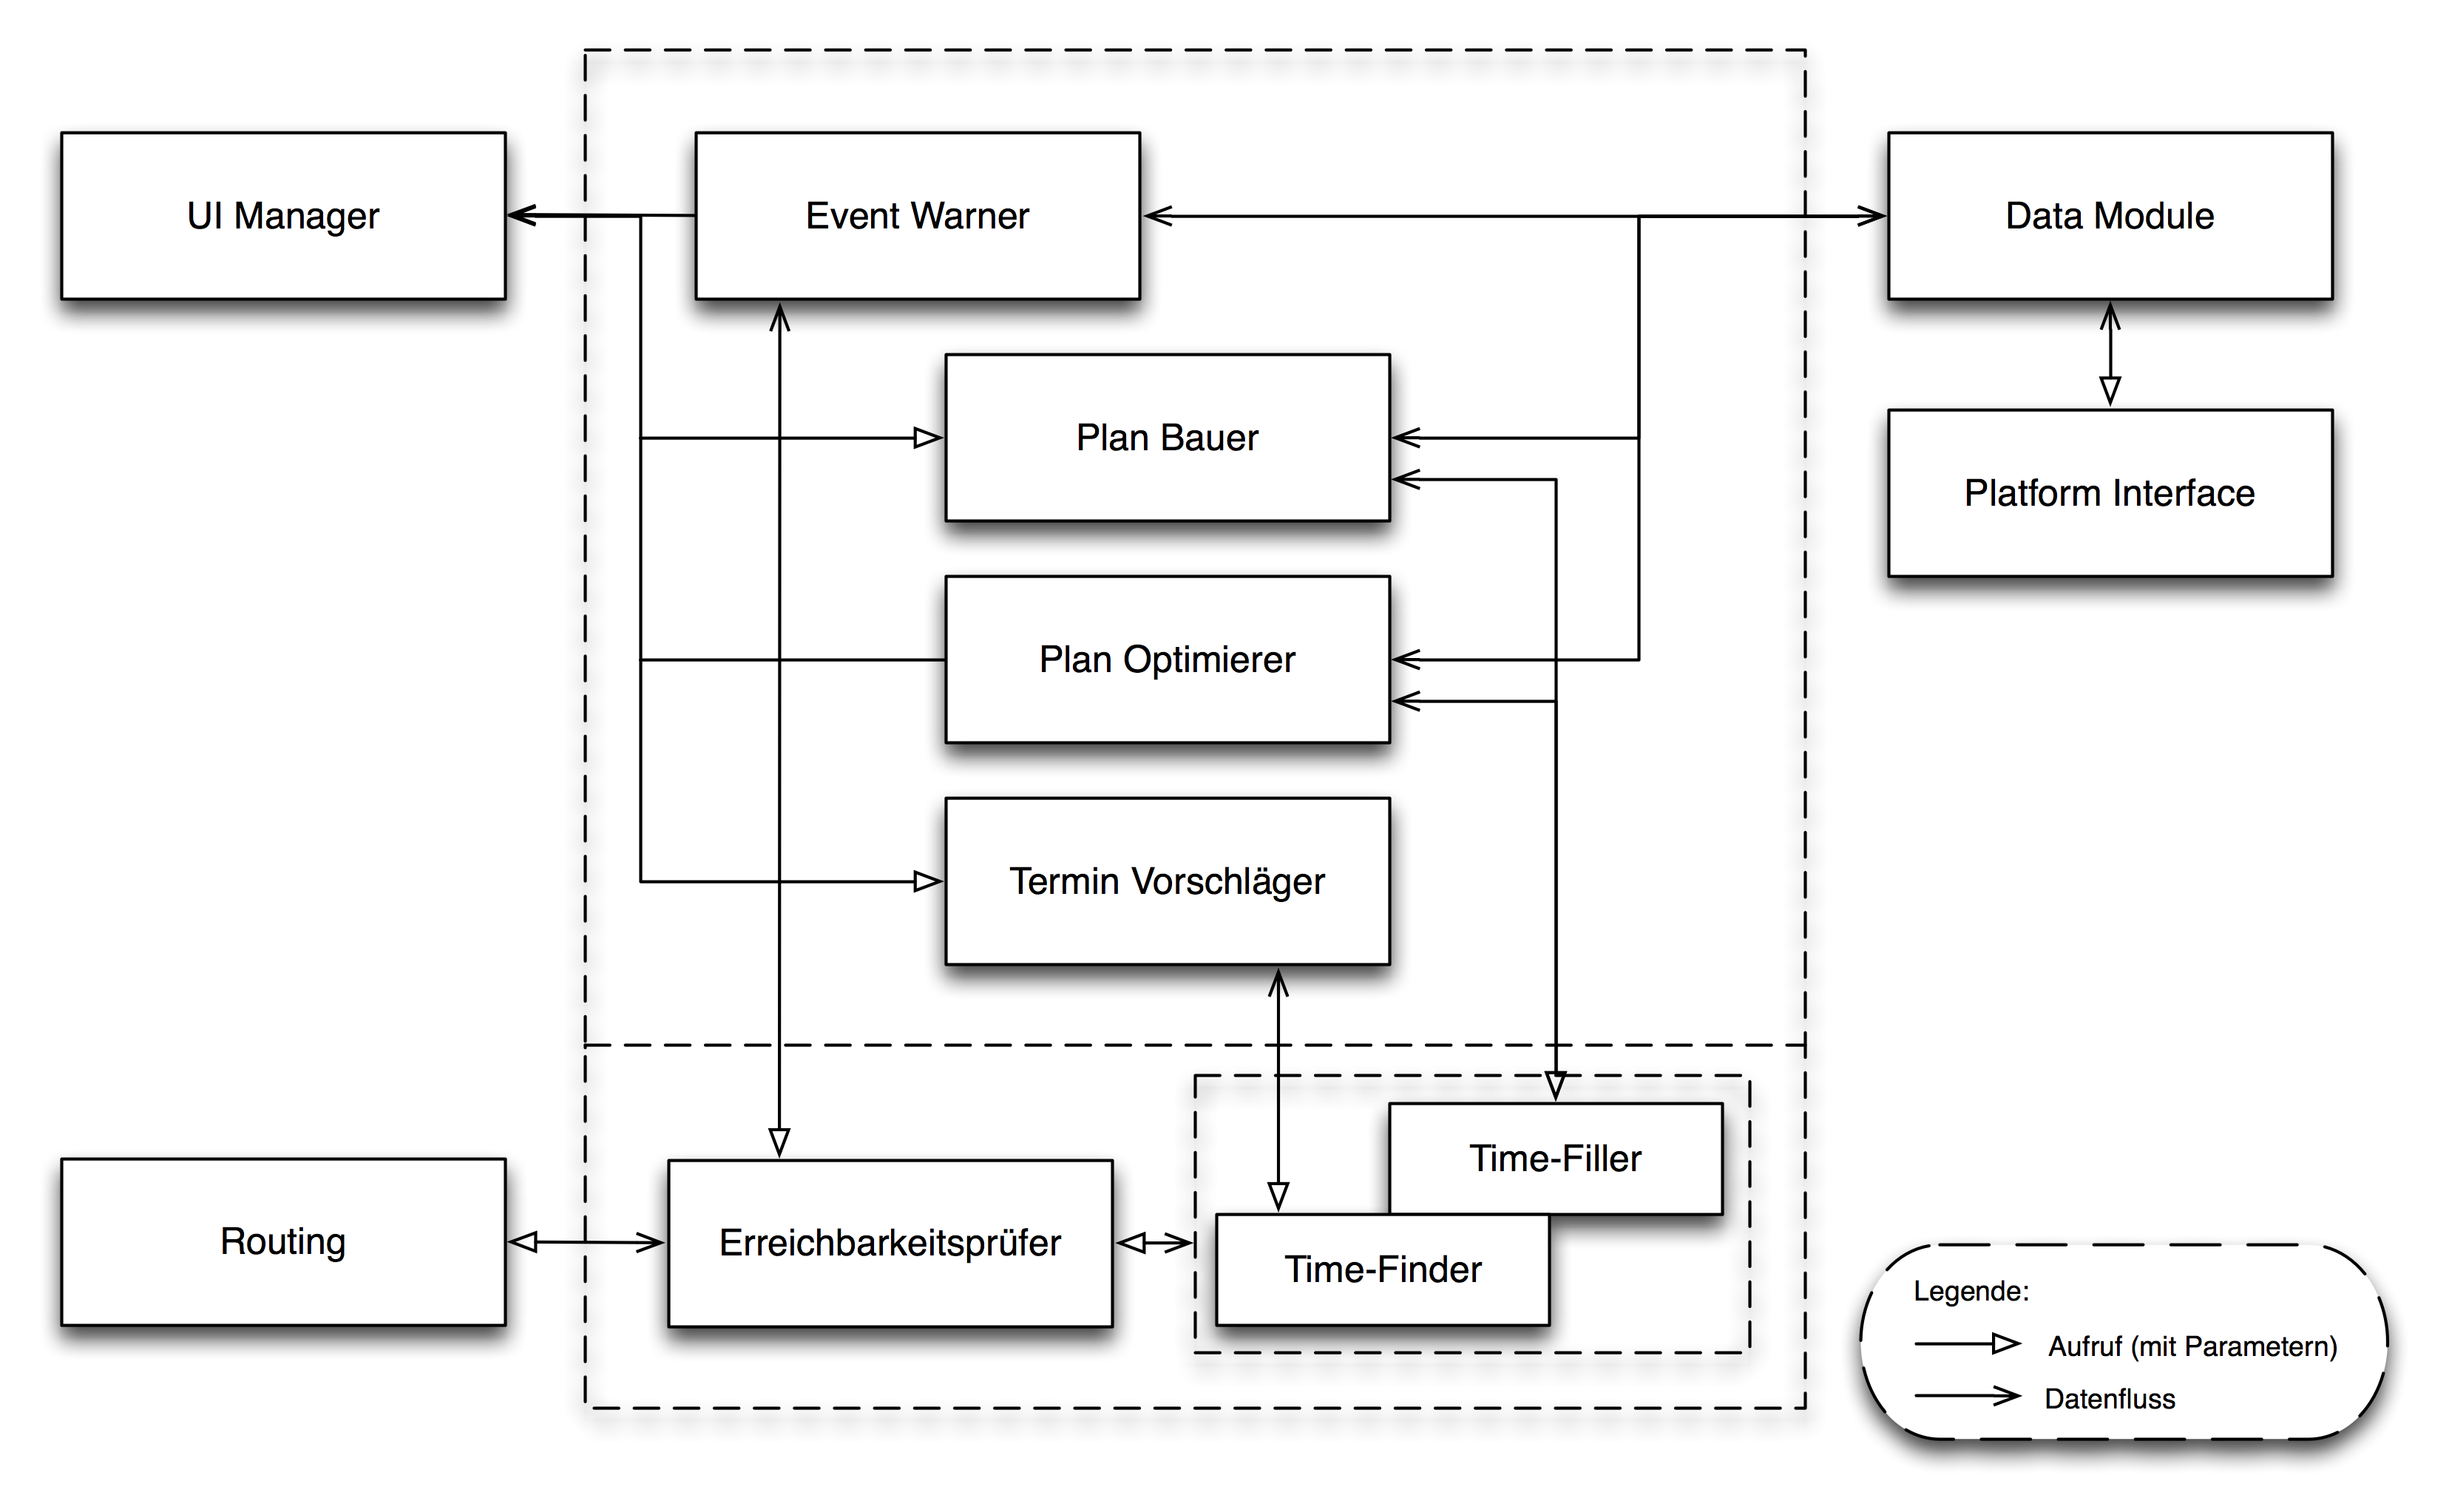
\includegraphics[width=16cm]{pics/event_stuff.png}
\caption{Components of the Appointment/Task optimization and verification engine}
\label{event_stuff}
\end{figure}

%\begin{figure}[h!]
%\centering
%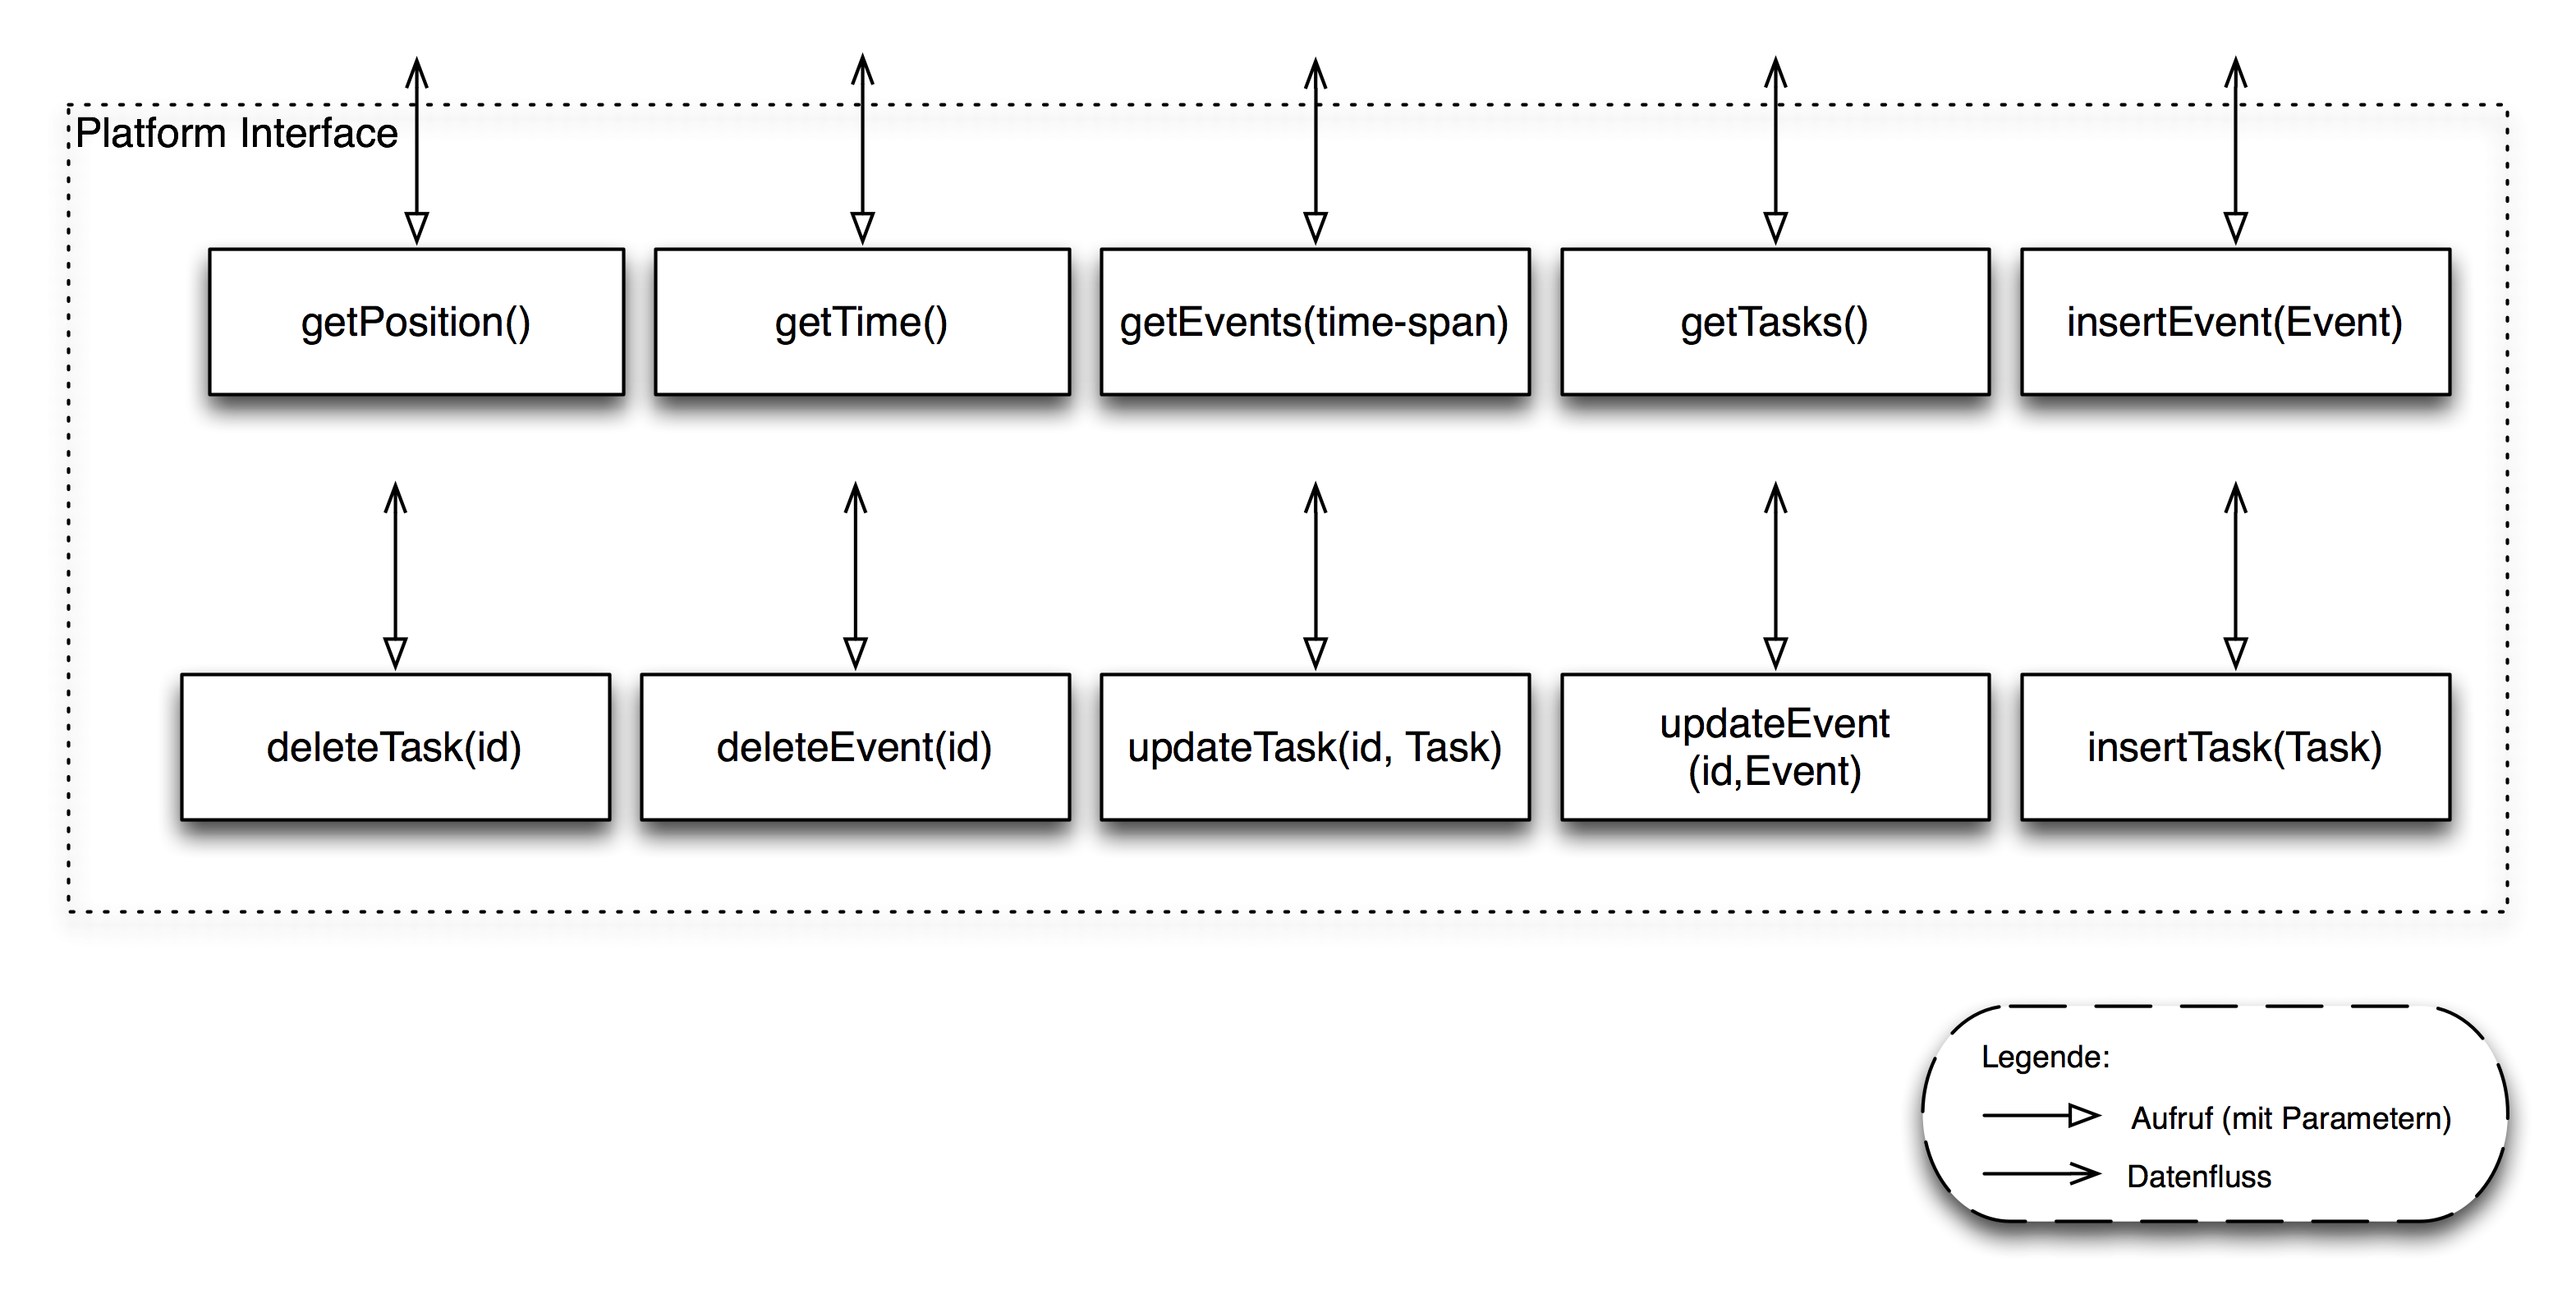
\includegraphics[width=16cm]{pics/data_module.png}
%\caption{Highlevel interface for data storage and system interaction}
%\label{gantt1}
%\end{figure}